\subsection{Block Diagram}
The block diagram is shown in Figure ~\ref{bd}.
\begin{figure}[H]
    \centering
    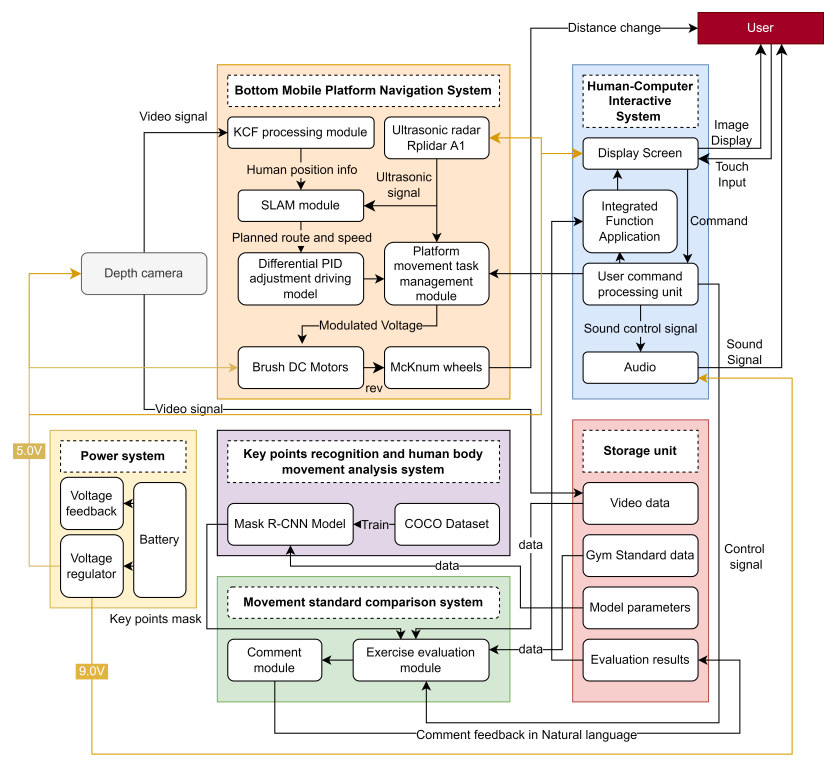
\includegraphics[width=13.5cm,height=12.5cm]{sections/Block.png}
    \caption{Block diagram}
    \label{bd}
\end{figure}


\subsection{Subsystem Overview}
\subsubsection{Bottom mobile platform programming and hardware setting}
We plan to take use of the ROS platform as the base movement platform of the robot. This robot platform contains two ultrasonic radars, steering gear and steering gear control system. The control system can be connected to the outer host to program more detailed movement assignments. We will use the camera to capture human's image, and use KCF algorithm to calculate the navigate task information for the steering gear, and then the robot can follow behind the human. We expect that the robot to work on a flat surface, not a rough dirt road. Some obstacles are allowed around the robot, and the robot will
avoid them. In addition, other hardware components of our project include the display, the speaker, the control console and the camera. 
\subsubsection{Key points recognition and movement analysis of the human body}
The most important part of this program is that we will use the Mask R-CNN to do the skeletal binding and key points recognition to determine the human’s body movement status. When the robot is working, it will first record people's exercise as a video file. Then, it will analyze it to decide how it fits with the standard. In this step, we require the exerciser to do the exercise in the specified orientation. For example, during the squat, we ask the exerciser to face with the robot; during sit-ups, the user should turn the side towards the robot to facilitate movement analysis. 
\subsubsection{Movement standard algorithms}
One important part in this research is that how we decide whether the exercise is ``good" or not. For the sports like Chinese middle school broadcast gymnastics, we have a systematic evaluation system, in which we will mark the movement of the user and count the number of the standard movement they make. In such a rhythmic movement, we will use the speaker to play rhythm music or feedback. For such exercises as push-ups, and squats, in addition to detecting whether the corresponding movements are in place, we also need to count the number of a complete round of movements the user has already done.
\subsubsection{Man-machine interactive system}
All of the above mentioned functions will be integrated into a user-friendly program. In the robot's human-computer interaction platform, we hope that different functions can be freely converted by users, and the output information can also be amateur-friendly.


\newpage
\subsection{Subsystem Requirements}
\subsubsection{Bottom mobile platform programming and hardware setting}
The tracking is required to work with the following rules: 1) When the distance is larger than 3 meters, the robot will start moving; the larger distance is, the higher the motor power is, and with an upper speed limitation. 2) The robot will stop when the distance is smaller than 2 meters. 3) When the user actively approaches the robot, the robot will not go backward. 4) When the robot’s tracking program is activated, if no one is in front of the camera, it stays still until someone comes into view; the robot will use the first person it sees as the target to track and movement analyzing, while ignoring other people who come into view later. 5) If there are multiple people in view at startup, it will pick the nearest person as its target. 6) If the target quickly runs out of view, it will stay still until a new target appears.

The hardware utilized on the mobile platform should be assembled and compatible with each other. For one aspect, all hardware devices, including the screen, speaker, camera, etc. should be firmly and aesthetically appropriately installed onto the EAI SMART platform, and in that case, we need to make a steel frame to give the robot a reasonable shape and attach the hardware to the upper frame. For another, the connection and interaction between hardware components have to be smooth and robust, since information from one part need to be spread to the next few parts as ``igniter" or ``guide".
\subsubsection{Key points recognition and movement analysis of the human body}
This subsystem will use framework such as Mediapipe to recognize human skeleton and joints. Besides, when the certain movement is given to the robot, it needs to move to an appropriate position for recording videos: having a distance of around 2 meters with the exerciser. Another factor to be taken into consideration is the time of analyzing the recorded video; we require approximate 1 minute or 2 for each individual movement and more for a set of movements.
\subsubsection{Movement standard algorithms}
We need to design respective algorithms for different movement categories so as to evaluate whether the user is doing the exercise in a standard manner. Considering the push-up, the algorithm should emphasize that the limbs and joints need to be moved to a specified angle and position at a specified point of time. Considering the individual movements, it is necessary for our algorithm to be more flexible in counting the number of movement of the exercisers and whether a period of movement is up to standard.
\subsubsection{Man-machine interactive system}
We plan to perform the interaction based on a touchpad, and thus the data transfer is required to be quick and lossless. For example, the recording and analyzing of videos need to be able to pulse or cease at arbitrary time. Furthermore, the main information of each interface should be clearly and conspicuously shown to the exerciser, like showing the movement name and time count with large font when recording the exercising videos.


\subsection{Subsystem Verifications}
\subsubsection{Bottom mobile platform programming and hardware setting}
To verify the hardware components, we can simply check whether ports can be directly inserted and removed from the data cable without disassembling other hardware components, and whether the frame of the vehicle can move steadily without shake during the driving process.

To verify the tracking functionality of the robot, we can test by guiding the robot to move by ourselves, and measure the distance and speed of the robot as it tracks us. We can check if the robot keeps a distance with the user in a range of 2 to 3 meters, goes backward when the user approaches, and turning left/right if the user does so. With two team members for testing, we can also verify that the robot picks the nearest person as the target at startup, and stays still until a new target appears if the current target runs out of view. If the robot behaves as expected in these testing tasks, we can conclude that the tracking functionality meets the requirements.
\subsubsection{Key points recognition and movement analysis of the human body}
Verify skeleton and joint recognition accuracy by testing the subsystem on a variety of human movements and measuring its precision, recall, and F1 score.

Verify robot positioning accuracy by testing the subsystem with different movement scenarios and measuring the distance between the robot and exerciser to ensure it's around 2 meters.

Verify video analysis time by testing the subsystem on videos of different lengths and ensuring it can analyze individual movements within 1-2 minutes and longer videos proportionally.
\subsubsection{Movement standard algorithms}
Verify movement category algorithms by testing their accuracy and robustness on a dataset of videos, measuring precision, recall, and F1 score.

Verify push-up algorithm by testing its accuracy in detecting the correct angles and positions on a dataset of push-up videos, measuring mean absolute error and root mean square error.

Verify individual movement algorithm by testing its flexibility and accuracy in detecting the correct number of movements and evaluating their standards on a dataset of exercise videos, measuring accuracy and F1 score.
\subsubsection{Man-machine interactive system}
We can verify the quick and lossless data transfer by measuring the transfer speed and checking for lost or corrupted data packets. If the transfer speed is fast and no data is lost or corrupted, conclude that the data transfer meets the requirements.
We can verify the ability to pulse or cease video recording and analysis at arbitrary times by performing tests where we manually start and stop the functions. If the functions can be activated and stopped without any issues, conclude that the system meets the requirements.
We can verify the clear and conspicuous display of interface information by testing it with exercisers and collecting feedback. If the feedback is positive and the displayed information is clear and conspicuous, conclude that the interface design meets the requirements.


\subsection{Tolerance Analysis}
Achieving success in our project depends on the continuity of camera-captured photos as the inputs to our model. However, unlike some of the dataset collected by surveillance camera, which is super steady, there might be vibrations in our camera input. Besides, in real-life scenarios, the road may not always be super flat, leading to non-continuous images with significant gaps in a short period. Such unstable images present a challenge when stitching them together to form the whole picture. Misalignment of the same lines in these images can result in distortions, leading to a poorly reconstructed image that is twisted and of low quality.

Another potential problem is how can we deal with the case where there are more than one people in the image. Our model should be able to identify the user we have been tracking and ignore others while not hitting them. Our tracking system should be able to handle those challenges, we will design an algorithm to stabilize the image and provide steady inputs to model, and as for the multiple people case, we think one possible approach is to train our model with test cases with several people. After correctly labeling the people in sight, we could try track our user by putting him in the center of sight.

Besides, During the recognition and analysis of human body movements, occasional errors in key point recognition may occur, potentially affecting the accuracy of movement analysis. In such cases, it is essential that the Mask R-CNN algorithm is robust enough to handle missing or inaccurately detected key points effectively. One possible solution is to incorporate data augmentation techniques during the training of the Mask R-CNN model, such as rotation, scaling, or flipping, to improve its generalization capabilities and tolerance to variations in human body movements. Another possible approach is to leverage ensemble learning techniques, such as stacking multiple models or using model averaging, to improve key point recognition accuracy and robustness. 

The tolerance limits we set for the object tracking algorithm is:
\begin{enumerate}
    \item Mask R-CNN accuracy: Minimum 95\% accuracy in key point recognition.
    \item Positioning accuracy: ±0.2 meters from the desired 2-meter distance.
\end{enumerate}

\newpage